\documentclass{article}
\usepackage[a4paper, total={7in, 9in}]{geometry}
\usepackage{tikz}
\usepackage{fancyhdr}
\usepackage{amssymb}
\title{$\aleph_0$   ...  $\aleph_1$}
\author{Elijah Williams}
\date{29 August, 2023}
\begin{document}
\pagestyle{fancy}
\fancyfoot[RO, RE]{Elijah D. Williams, Ben-Yaakov}
\maketitle
\newpage
\begin{large}
\begin{center}
  {\Huge Aleph Comparisions}
\end{center}





In discrete mathamatics, items can be grouped together in unordered list called sets.
A set can be any group of non-repeating objects.
For example a set called pets can be
\begin{center}
$ P = \{Dogs, Cats, Hamsters, Snakes\}$ 
\end{center}
While another set of jeresy numbers on sports teams can be
\begin{center}
$ N = \{0, 12, 6, 3, 23, 7, 5\}$

\end{center}
These two list are considered sets because there order does not matter, and they do not have repeating elements.
We can talk about the number of non-repeating elements in these sets using the word cardinality.
Cardinality is the word we use to describe the number of elements in each set.
We use vertical bars around the label of a set to denote its cardinality.
For example, the cardinality of the set of pets is 4, and the cardinality of the set of jeresy numbers is 7.
\begin{center}
  $ |P| = 4$
  \\
  $ |N| = 7$
  \\
\end{center}



     These two sets are finite, with a limit on elements, so have finite cardinalities.
However, not all sets are finite like this.
For example the set of rooms in a infinite hotel is a infinite (non finite) set with a different type of cardinality.
The cardinality for the other sets were specific natural whole numbers, with explicit values such as 4 or 7.
This is because they had an explicit finite amount.
However a infinite set like that of the rooms in an infinite hotel has a cardinality of $ \aleph_0 $ (aleph zero), or the entire set of natural numbers.
\begin{center}
  $ Infinite Hotel Rooms \rightarrow I = \{1, 2, 3, 4, 5, 6, ... \infty\}$
  \\
  $ |I| = \aleph_0 $
\end{center}


\begin{center}
  *note aleph or aleph zero is not the same as infinity
  $ \aleph  \neq \infty $
  \\
\end{center}
Aleph and infinity are not the same.
Aleph is character value, specifically used to show the cardinality of sets.
While infinity is used as an extreme limit or a sequence that increases without bounds.
\\


     Aleph has several variatioons, like the previously shown $ \aleph_0$ (aleph zero) used to denote the cardinality of the smallest sets of infinity.
This variation has several names, such as aleph null, aleph nought or aleph zero.
A set of this cardinality can have a bijection (each member of each set can be mapped to an indivisual member of the other set)of the countably infinite set of all natural numbers.
\\

This set's cardinality is equivalent to all countably infinite sets, such as the set of all integers, primes, squares, odds, evens, and square roots.
All of these sets have a cardinality of $ \aleph_0$ due to their countably infinite nature.
The next smallest cardinality of aleph is $ \aleph_1$ which is equivalent to the cardinality of the smallest uncountably infinite set.
This variation is equivalent to the cardinality of the set of real numbers, or the continuum.
The infinite set of real numbers is determined to have a larger cardinality than that of natural numbers, because there is no bijective function mapping real numbers to natural numbers, and the set of natural numbers is a subset of real numbers.
\\


      The set of natural numbers being a subset of real numbers is self-explanatory, however the set of real numbers not being bijective to natural numbers is not.
For example earlier the statement was made that the set of natural number's cardinality is equivalent to that of the set of primes, and integers.
This seems false due to the set of primes being a subset of naturals, which is a subset of integers.
Which  is true yet, a function mapping any two of the sets can be bijective.
For example with integers, you can map all the negative integers to all odd natural numbers, and positive integers to even natural numbers to make a bijective function mapping naturals, to integers.
\\
\\
\begin{center}
  {\huge$ \mathbb{N} \leftrightarrow \mathbb{Z}$}
  \\
  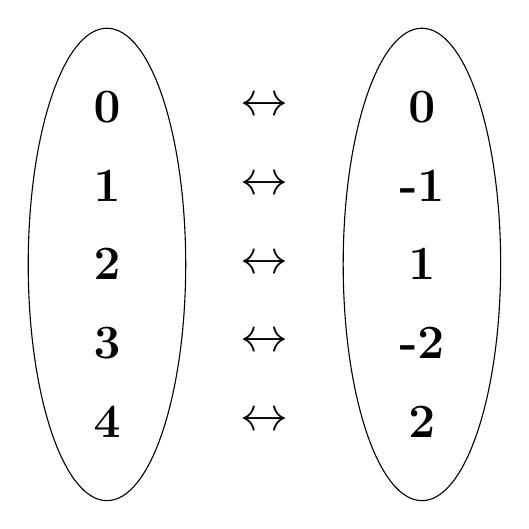
\begin{tikzpicture}
    \draw (2,5) ellipse (1cm and 3cm);
    \node at (2,3) {\LARGE\textbf{4}};
    \node at (6,3) {\LARGE\textbf{2}};
    \node at (4,3) {\LARGE\textbf{$ \leftrightarrow$}};
    \node at (2,4) {\LARGE\textbf{3}};
    \node at (6,4) {\LARGE\textbf{-2}};
    \node at (4,4) {\LARGE\textbf{$ \leftrightarrow$}};
    \node at (2,5) {\LARGE\textbf{2}};
    \node at (6,5) {\LARGE\textbf{1}};
    \node at (4,5) {\LARGE\textbf{$ \leftrightarrow$}};
    \node at (2,6) {\LARGE\textbf{1}};
    \node at (6,6) {\LARGE\textbf{-1}};
    \node at (4,6) {\LARGE\textbf{$ \leftrightarrow$}};
    \node at (2,7) {\LARGE\textbf{0}};
    \node at (6,7) {\LARGE\textbf{0}};
    \node at (4,7) {\LARGE\textbf{$ \leftrightarrow$}};
    \draw (6,5) ellipse (1cm and 3cm);
  \end{tikzpicture}
\end{center}

     This  remapping of the sets to create a bijective function between them is not possible between natural numbers and real numbers, due to the unique nature of real numbers, not needing to terminate.
This means you can use cantors diagonal argument(an argument stating there is no complete list of real numbers, due to the ability to take one digit from each member of the list and change it to create a number not listed on the list) to prove the set of reals is greater than that of the set of naturals.
\\

      Due to the axiom of choice, you can deduce that there is no seperate cardinality between these two seperate sized sets, of $ \aleph_0 $  (aleph zero) and$ \aleph_1 $ (aleph one).
The axiom of choice has the concept of ordering sets, for example from small to big.
You can do this from natural numbers counting up from zero or one.
With this ordered infinite set, you can start mapping them to real mumbers, and you will quickly see that the mapping will always be off.
For example if you map $0_n -> 0_r$ and then $ 1_n -> 0.1$, you will always be able to add a zero before the last digit, making an infinite sequence, just between the first two natural numbers.
This shows the difference between aleph one and aleph zero as just an order of power.
$ \aleph_1 = 2^\aleph$ Aleph one equeals two to the aleph null.
With there being no possible in between as this is smalle than $\aleph^2$ yet still greater than $\aleph$

      

\end{large}
\newpage
\begin{Huge}
{\center \section{Citing}}
\end{Huge}
\begin{large}
  Lewis, H. R., and Zax, R. $ (2019) $. Essential discrete mathematics for computer science.
  \\
        Princeton University Press.
\\
Poonen, B., and, N. $ (2002) $. INFINITY: CARDINAL NUMBERS.
     https://mathcircle.berkeley.edu/sites/default/files/BMC5/docpspdf/infinity.pdf
\\
The editors of encyclopadia of Britanica. $ (n.d.) $. Aleph-null | Definition, Transfinite
       Numbers, Infinity, and Facts | Britannica. Www.britannica.com. Retrieved
       December 5, 2023, from https://www.britannica.com/science/aleph-null
       \\
       Vanderbuilt University, The Axiom Of Choice
       https://math.vanderbilt.edu/schectex/ccc/choice.html
       \\
University of Kansas, Cantor's Diagonal argument.
     https://jlmartin.ku.edu/courses/math410-S09/cantor.pdf
     \\
 %    \footnote {


     
     

\end{large}
\end{document}
